\documentclass[12pt]{article}

\usepackage[utf8]{inputenc}
\usepackage{geometry}
\geometry{a4paper,scale=0.75}
\linespread{1.5}
\usepackage{graphicx} 
\usepackage{float} 
\usepackage{subfig} 
\usepackage{enumerate}
\usepackage{enumitem}
\usepackage{amsmath}
\usepackage{array}
\usepackage{booktabs}
\usepackage{multirow}
\usepackage{amsfonts}
\usepackage[english]{babel}
\usepackage{amsthm}
\usepackage{dcolumn}
\usepackage{multicol}
\usepackage{stfloats}
\usepackage{lscape}
\usepackage[figuresright]{rotating}
\RequirePackage{pdflscape}
\usepackage[toc,page]{appendix}
\usepackage{geometry}
\usepackage{longtable}
\usepackage{comment}
\usepackage{xcolor}

% -------- enumerated sub-labels (a), (b), … --
\usepackage{enumitem}
\setlist[enumerate,1]{label=(\alph*),ref=\alph*}
% ---------------------------------------------

\usepackage{hyperref}
\hypersetup{hidelinks,
	colorlinks=true,
	allcolors=black,
	pdfstartview=Fit,
	breaklinks=true}
\usepackage{csquotes}
\usepackage{natbib}
\bibliographystyle{apalike}
\newtheorem{definition}{Definition}
\newtheorem{theorem}{Theorem}
\newtheorem{proposition}[theorem]{Proposition}
\newtheorem{lemma}[theorem]{Lemma}
\newtheorem{corollary}[theorem]{Corollary}
\newtheorem*{remark}{Remark}
\newtheorem{example}{Example}
\newtheorem{exercise}{Exercise}
\newtheorem{assumption}{Assumption}[section] % number within sections


\begin{document}

\begin{center}
    ECON 3123: Macroeconomic Theory I\\
    {\large \textbf{Tutorial Note 3: Investment and Financial Market}}\\
    Solution to Exercises\\
    Teaching Assistant: Harlly Zhou
\end{center}

\begin{enumerate}[label=\arabic*.]
    \item (1) D. (2) D.
    \item (1) B. (2) C. Government selling bond is like borrowing money from the citizens.
    \item C.
    \item The answer is as in the following table.
        \begin{figure}[htp]
            \centering
            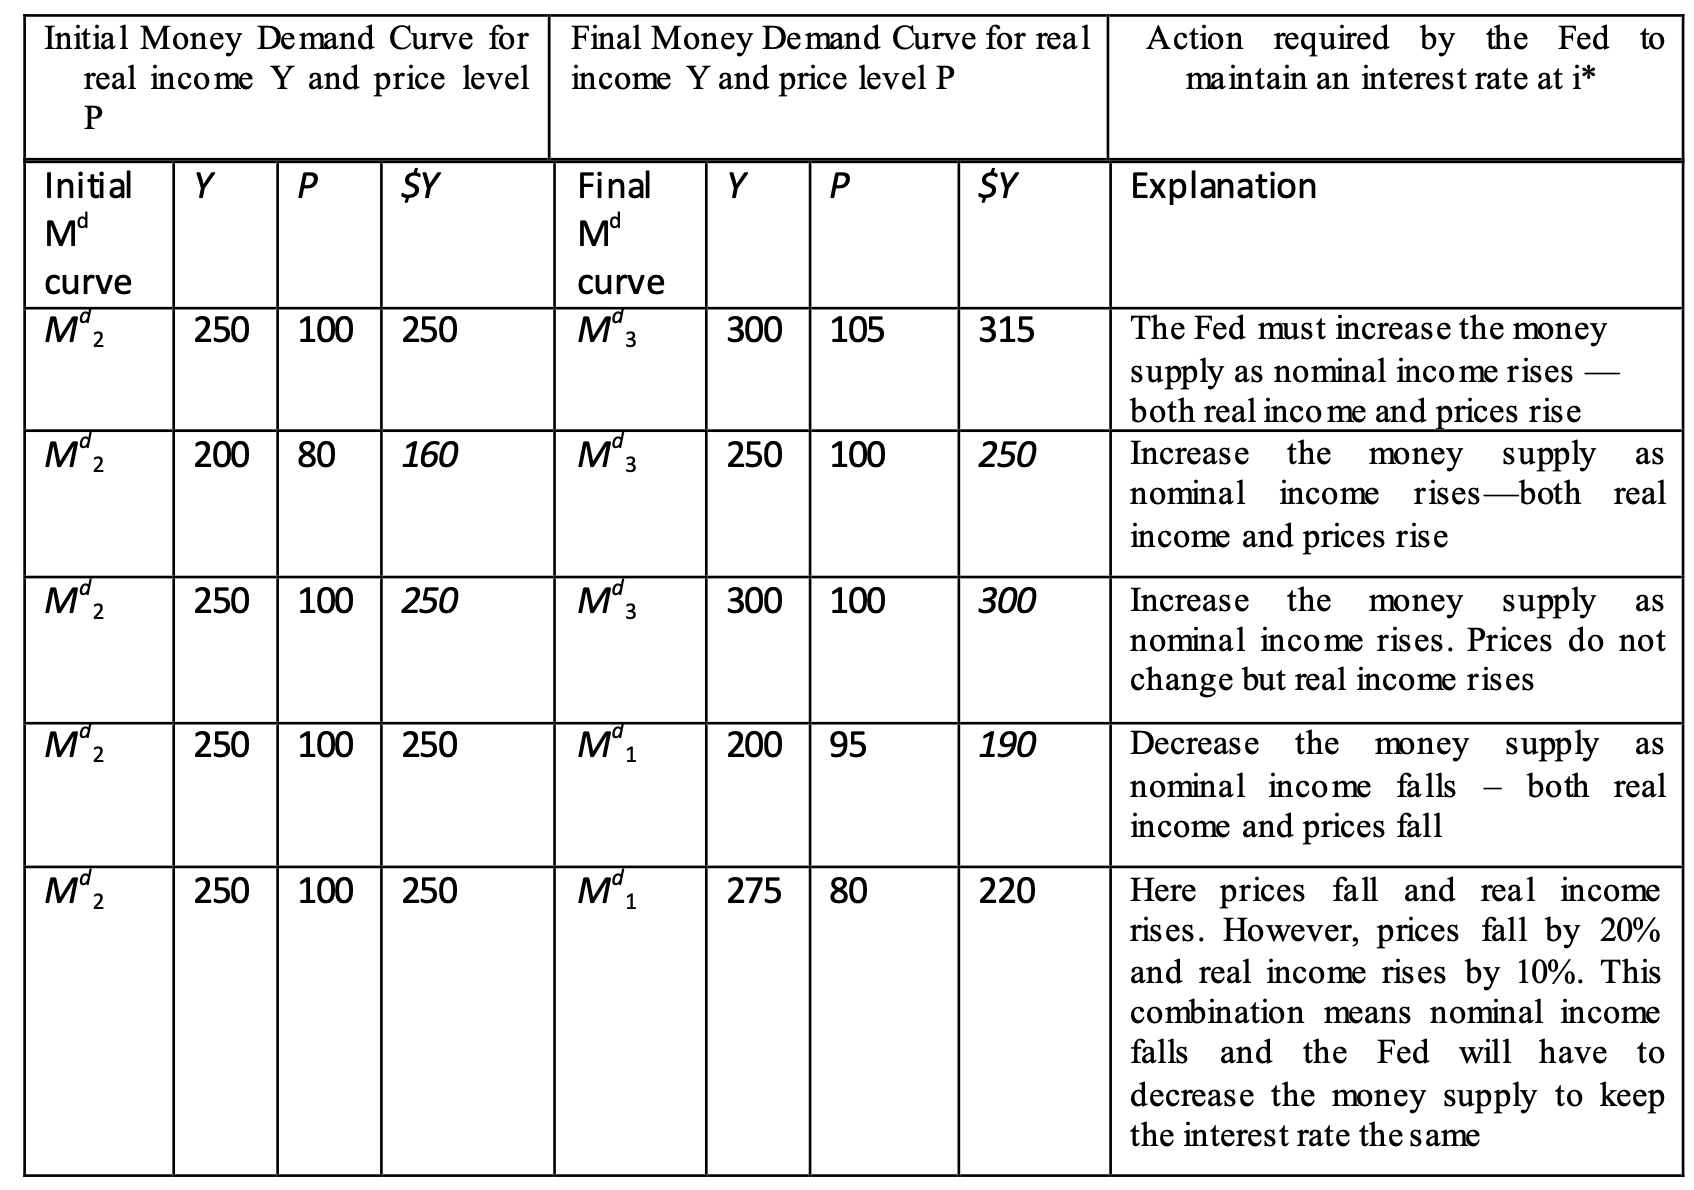
\includegraphics[width=0.8\textwidth]{ch4q9.png}
        \end{figure}
\end{enumerate}






\end{document}